\documentclass[14pt]{matmex-diploma}

\usepackage{graphicx}
\graphicspath{{teapot.png}}
\DeclareGraphicsExtensions{.pdf,.png,.jpg}

\begin{document}
\filltitle{ru}{
    chair              = {Математическое 
        обеспечение и администрирование информационных систем},
    title              = {Реализация алгоритма Ray Marching},
    type               = {coursework},
    position           = {студента},
    group              = 241,
    author             = {Гурьев Василий Александрович},
    supervisorPosition = {к.т.н., доц},
    supervisor         = {Литвинов Ю.В.},
}
\maketitle
\tableofcontents
\section*{Введение}
Компьютерная графика --- достаточно важный аспект современного мира. У нее много применений \cite{wiki:cg} 
и одно из них --- получение произвольных реалистичных 3D изображений. Обладая решеним данной задачи, так же 
решается и целый класс задач, посвященных генерации реалистичного видеоизображения и т.п.
\\
В данный момент существует 2 основных алгоритма генерации реалистичных 3D изображений. Первый, самый популярный,
использующийся во всех компьютерных играх, основывается на представлении объектов на сцене как множества 
треугольников (рис. 1), с которым в последствии работает видеокарта, преобразуя его в изображение.
Второй алгоритм, Ray Tracing, заключается в том, что для каждого пикселя изображения пускается луч в сторону сцены 
и ищется пересечение со всеми объектами на сцене. Подробнее см. \cite{wiki:rt}.
\\
Однако и у одного и у другого метода достаточно много недостатков, у Ray Tracing --- очень большое время получения картинки,
у метода с треугольниками --- высокая сложность рисования 3D-моделей. Поэтому было решено исследовать и реализовать сравнительно 
новый и не слишком популярный алгоритм, Ray Marching, появившийся около 8 лет назад.

\begin{figure}[t]
\label{triangle_teapot}
\centering
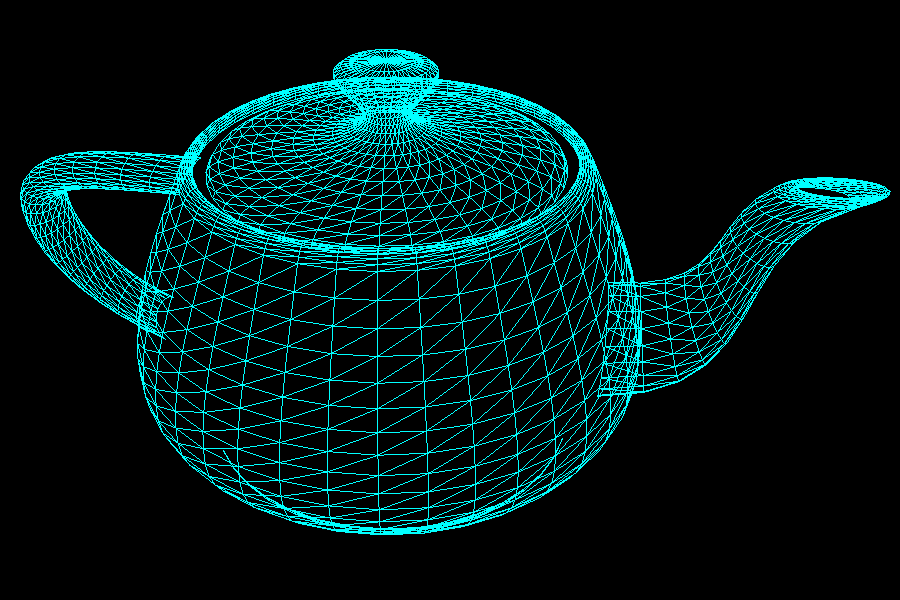
\includegraphics[width = 250pt]{teapot.png}
\caption{Пример объекта из треугольников}
\end{figure}

\section{Постановка задачи}
Итого было поставлено несколько задач: \\
1) исследование алгоритма Ray Marching; \\
2) реализовать данный алгоритм, а так же реализовать библиотеку с различными функциями Ray Marching-а; \\
3) реализовать IDE для сцен Ray Marching; \\
4) выполнить оптимизацию для выполнения сцен в реальном времени. \\

\section{Алгоритм}
Алгоритм Ray Marching в целом напоминает алгоритм Ray Tracing: из каждой точки изображения в сторону сцены пускается луч,
с помощью которого ищется пересечение с объектами, находящимися на сцене. Однако при использовании
Ray Tracing объекты в сцене заданы аналитически, причем пересечение ищется тоже аналитически. Например для
нахождения пересечения луча со сферой необходимо решить следующую систему уравнений~(\ref{система1}). 

\begin{equation}
\label{система1}
\begin{array}{rl}
x^2 + y^2 + z^2 & = R^2\\
(x - x_{0}) * x_{1} & = (y - y_{0}) * y_{1} = (z - z_{0}) * z_{1}
\end{array}
\end{equation}

При использовании же алгоритма Ray Marching объект в сцене задан как функция, для любой точки возвращающая 
наименьшее расстояние до этого объекта. Например объект
сферы, расположенной в точке (0, 0, 0) будет задан функцией~(\ref{функция1}). 

\begin{equation}
\label{функция1}
\begin{array}{ll}
float\,\,Sphere(vec3\,\,position,\, float\,\,radius)\\
\{                                                  \\
\,\,\,\,\,\, return\,\,length(position) - radios;   \\
\}                                                  \\
\end{array}
\end{equation}

Далее при помощи заданной функции идет итерация по лучу,
пущенному внутрь сцены. Более простым языком --- она вызывается сначала от самого начала луча, потом от точки, расположенной 
на расстоянии значения функции от начала луча по его направлению. Процесс продолжается до тех пор, пока не будет найдено пересечение,
или точка не выйдет за пределы сцены. Более наглядно это можно посмотреть на изображении (рис. 2)

\begin{figure}[t]
\label{ray}
\centering
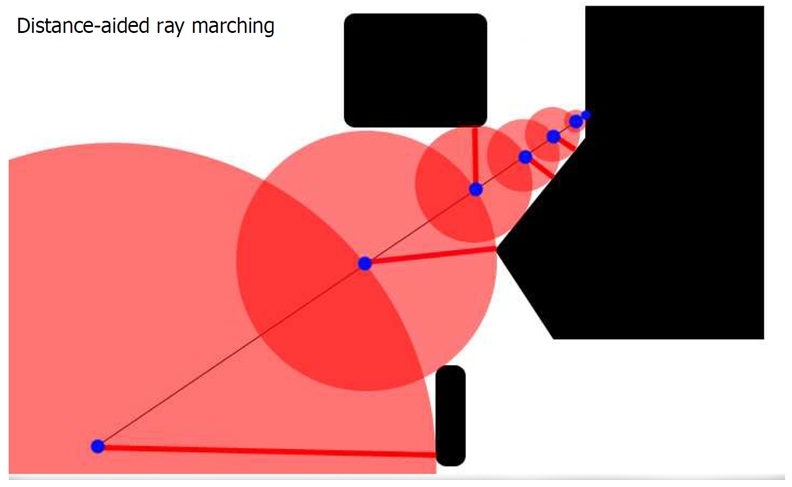
\includegraphics[width = 250pt]{ray.jpg}
\caption{Трассировка по лучу внутри сцены}
\end{figure}

\section{Некоторые примеры задания объектов}
В предыдущем пункте была рассмотрена функция, задающая сферу ~(\ref{функция1}). Теперь рассмотрим как пример функцию, задающую тор, расположенный в 
точке (0, 0, 0) ~(\ref{функция2}).

\begin{equation}
\label{функция2}
\begin{array}{ll}
float\,\,Torus(vec3\,\,pos,\, vec2\,\,rad)                                   \\
\{                                                                           \\
\,\,\,\,\,\, return\,\,length(vec2(length(pos.xz) - rad.x,\,pos.y)) - rad.y; \\
\}                                                                           \\
\end{array}
\end{equation}

Но функция из одного объекта это только самый простейший вариант задания сцены. 
Чтобы внутри сцены было несколько объектов, может быть применена функция для каждого из объектов, а затем взят минимум из результатов.
Такими же очевидними преобразованиями можно взять лишь пересечение 2 объектов, их разность и т.п. На следующем изображении (рис. 3) --- пример дома,
построенного при помощи алгоритма ray marching. Чтобы добиться такого эффекта,
было взято несколько вытянутых кубов и сделано из них нечто вроде завернутого тоннеля. Крыша --- те же приплюснутые повернутые кубы. Для представления 
окон из куба, играющего роль стены, каждые несколько <<метров>> были вычтены другой куб и сфера. 

\begin{figure}[h]
\label{house}
\centering
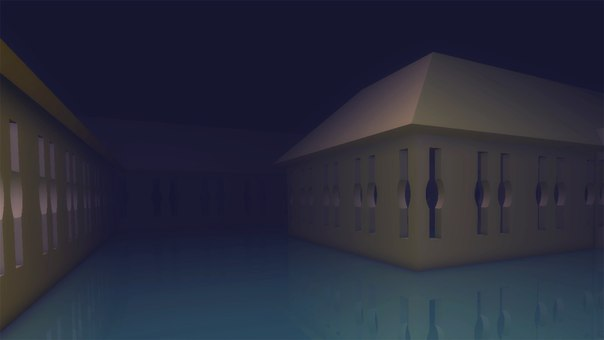
\includegraphics[width = 250pt]{house.jpg}
\caption{Объект <<дом>>, полученный различными операциями над простыми объектами}
\end{figure}

\section{<<Обычные>> эффекты}

На изображении (рис. 3) вы могли заметить, что у объекта присутствовал цвет, во всей сцене было освещение, отражение и тени.
В алгоритме ray marching когда было найдено пересечение с объектом в сцене можно возвращать не просто цвет объекта, с которым было найдено пересечение.
Можно посчитать нормаль в точке пересечения и, например с помощью модели освещения Фонга (\cite{wiki:fong}), вычислить освещенность в данной
точке учитывая источники освещения. Так же, зная нормаль, можно сделать мягкие тени, преломления, отражения и все те эффекты,
которые применяются в алгоритме ray tracing. А значит при помощи алгоритма Ray Marching может быть построена например данная сцена, построенная
при помощи ray tracing. (рис. 4)

\begin{figure}[h]
\label{ray tracing}
\centering
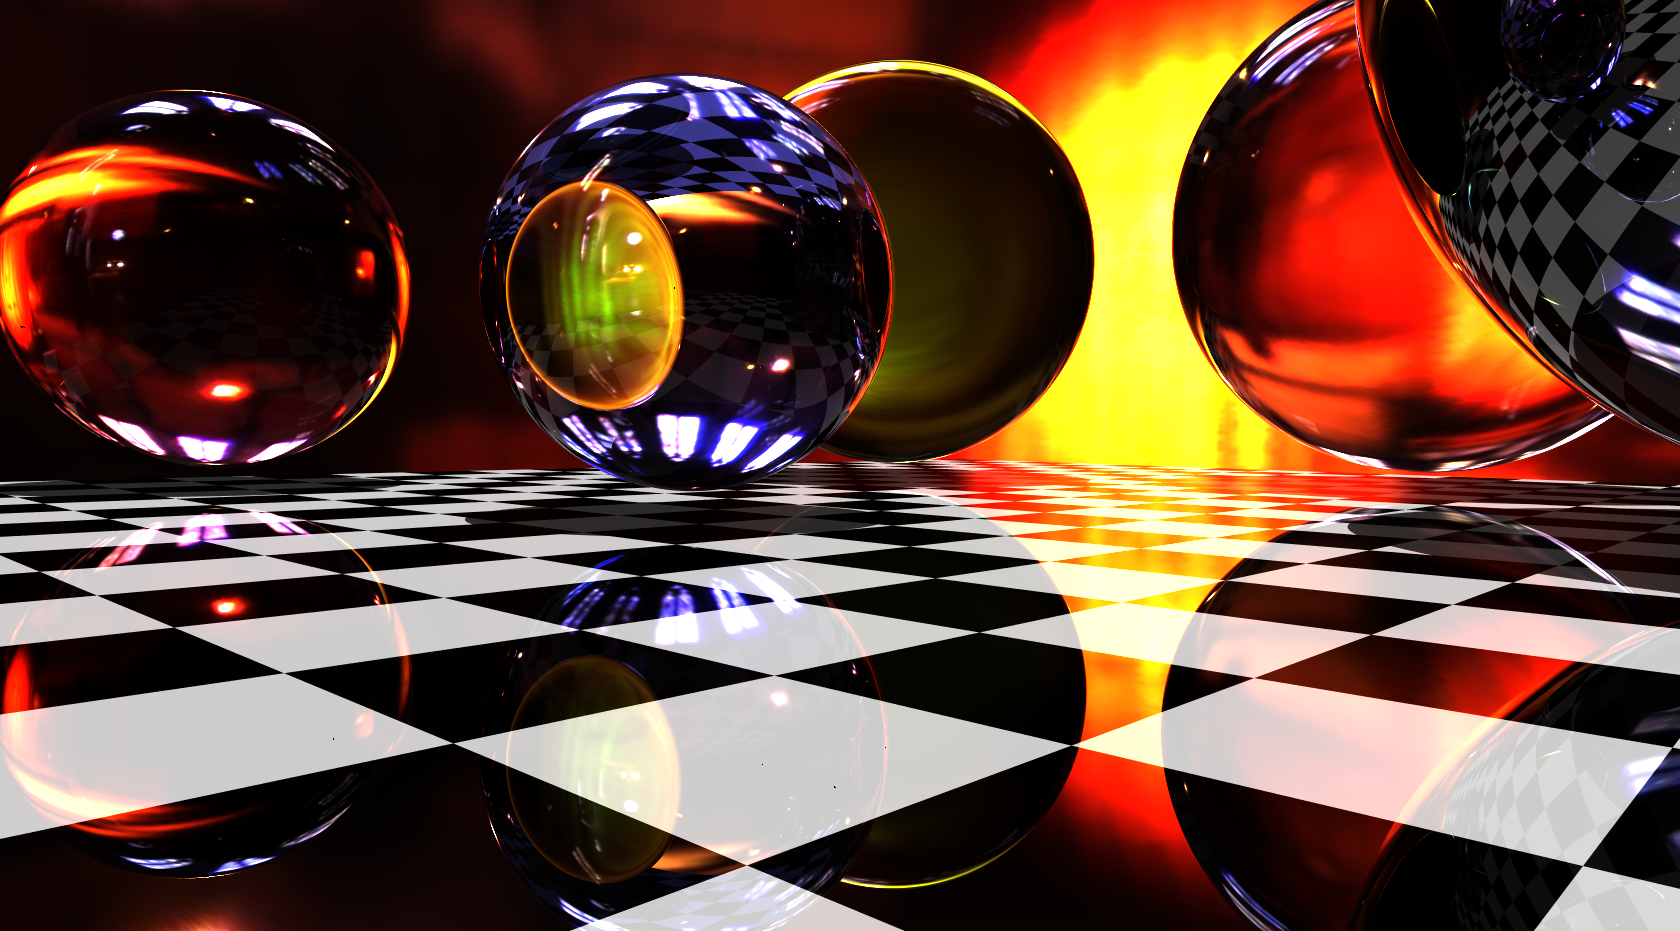
\includegraphics[width = 250pt]{scene.png}
\caption{Сцена ray tracing с различными эффектами}
\end{figure}

\section{<<Специальные>> эффекты}

Помимо привычных глазу эффектов освещения, теней и прочего, ray marching позволяет делать многое, что остальными алгоритмами получения
изображений сделать сложно, или даже вовсе невозможно. Будет приведено несколько примеров, сделанных при помощи реализованной IDE.
Первый пример --- репликация ~(\ref{функция3}).

\begin{equation}
\label{функция3}
\begin{array}{ll}
vec3\,\,opRep(vec3\,\,p,\,\,vec3\,\,c)         \\
\{                                             \\
\,\,\,\,\,\,return\,\,mod(p,\,\,c) - 0.5 * c;  \\
\}                                             \\
\end{array}
\end{equation}

Данная функция делит все пространство на параллелепипеды с диагональю <<с>> и располагает объект в середине каждого 
из этих параллелепипедов. Причем делается это лишь за одну операцию деления по модулю. В любом другом алгоритме сложность подсчетов увеличилось
бы многократно, соответственно вместе с этим производительность многократно бы уменьшилась. Пример действия данной функции в IDE можно посмотреть на изображении (рис. 5)

\begin{figure}[h]
\label{replace}
\centering
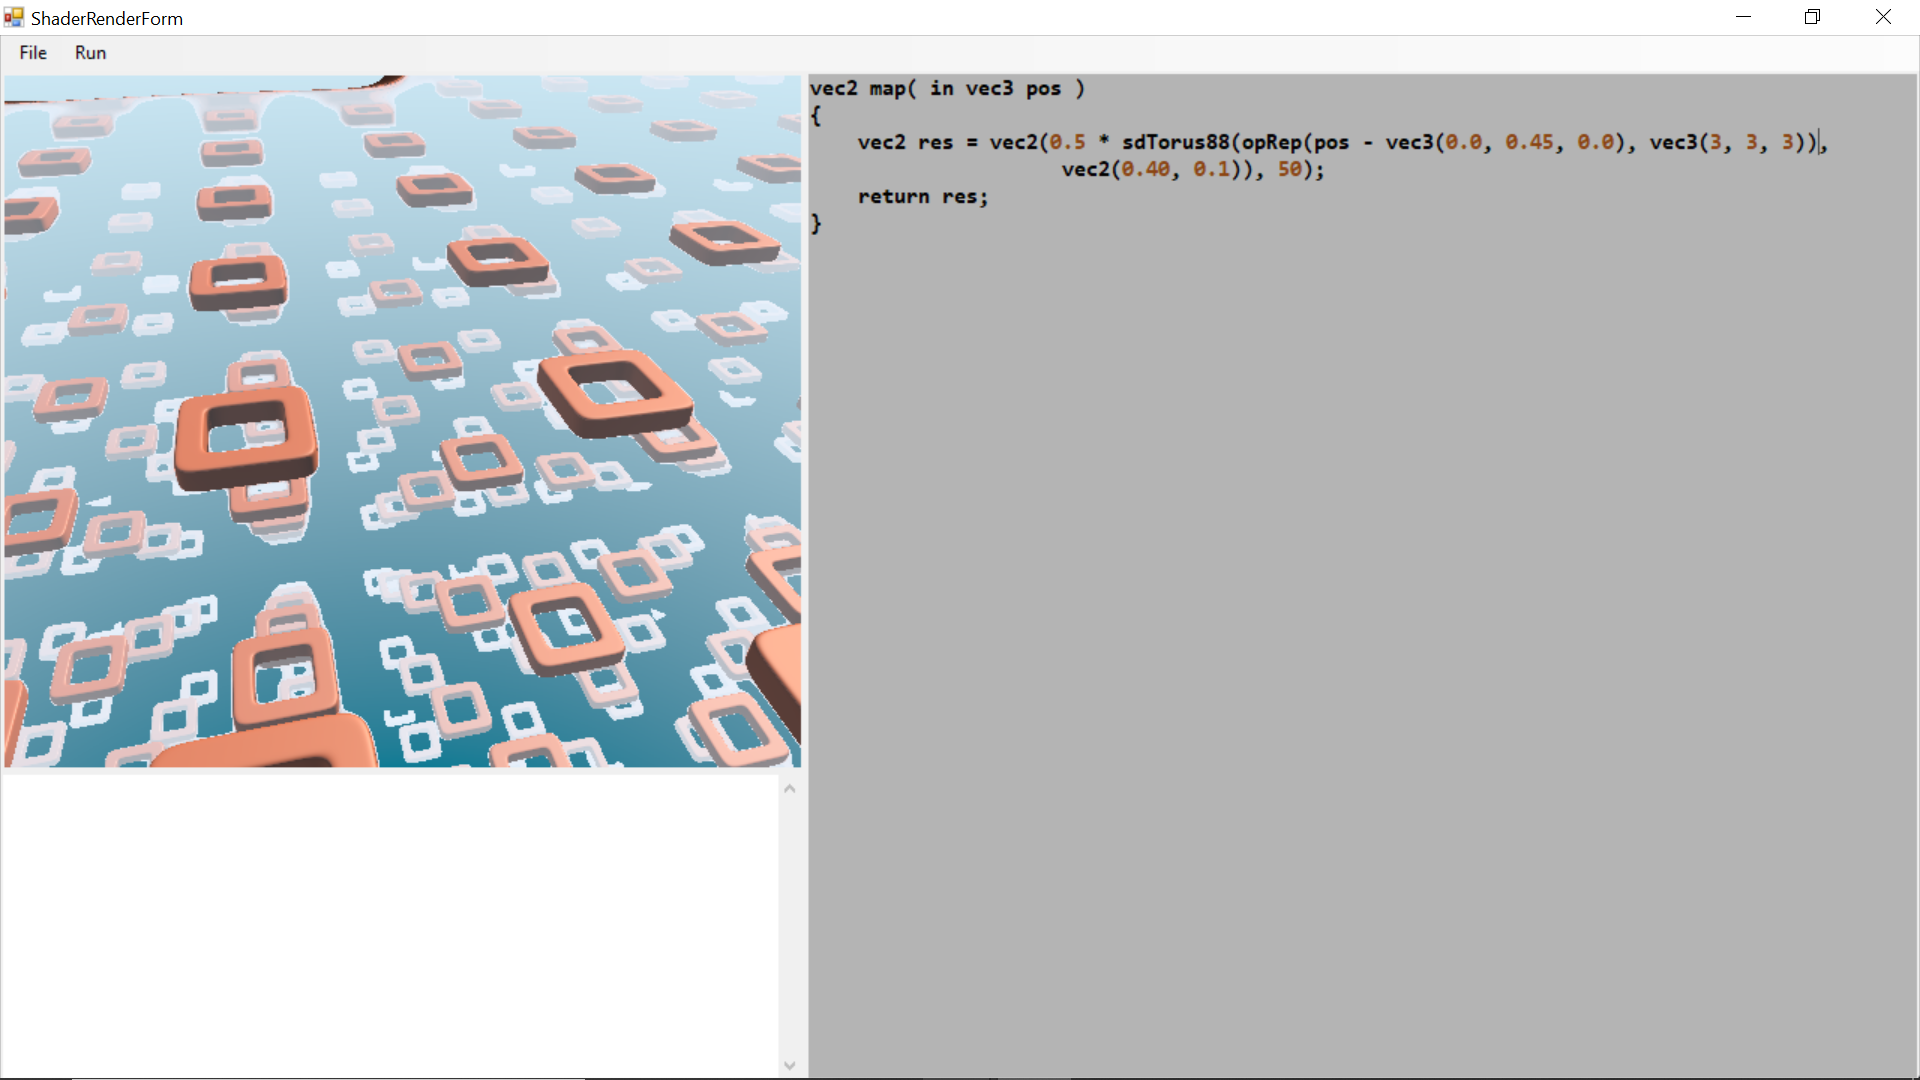
\includegraphics[width = 250pt]{replace.png}
\caption{Результат действия функции <<opRep>>}
\end{figure}

Следующий пример --- поворот всего объекта по спирали. Код данной функции можно посмотреть на Git, файл <<RayMarchBegin.glsl>>. 
Пример действия (рис. 6)

\begin{figure}[h]
\label{twist}
\centering
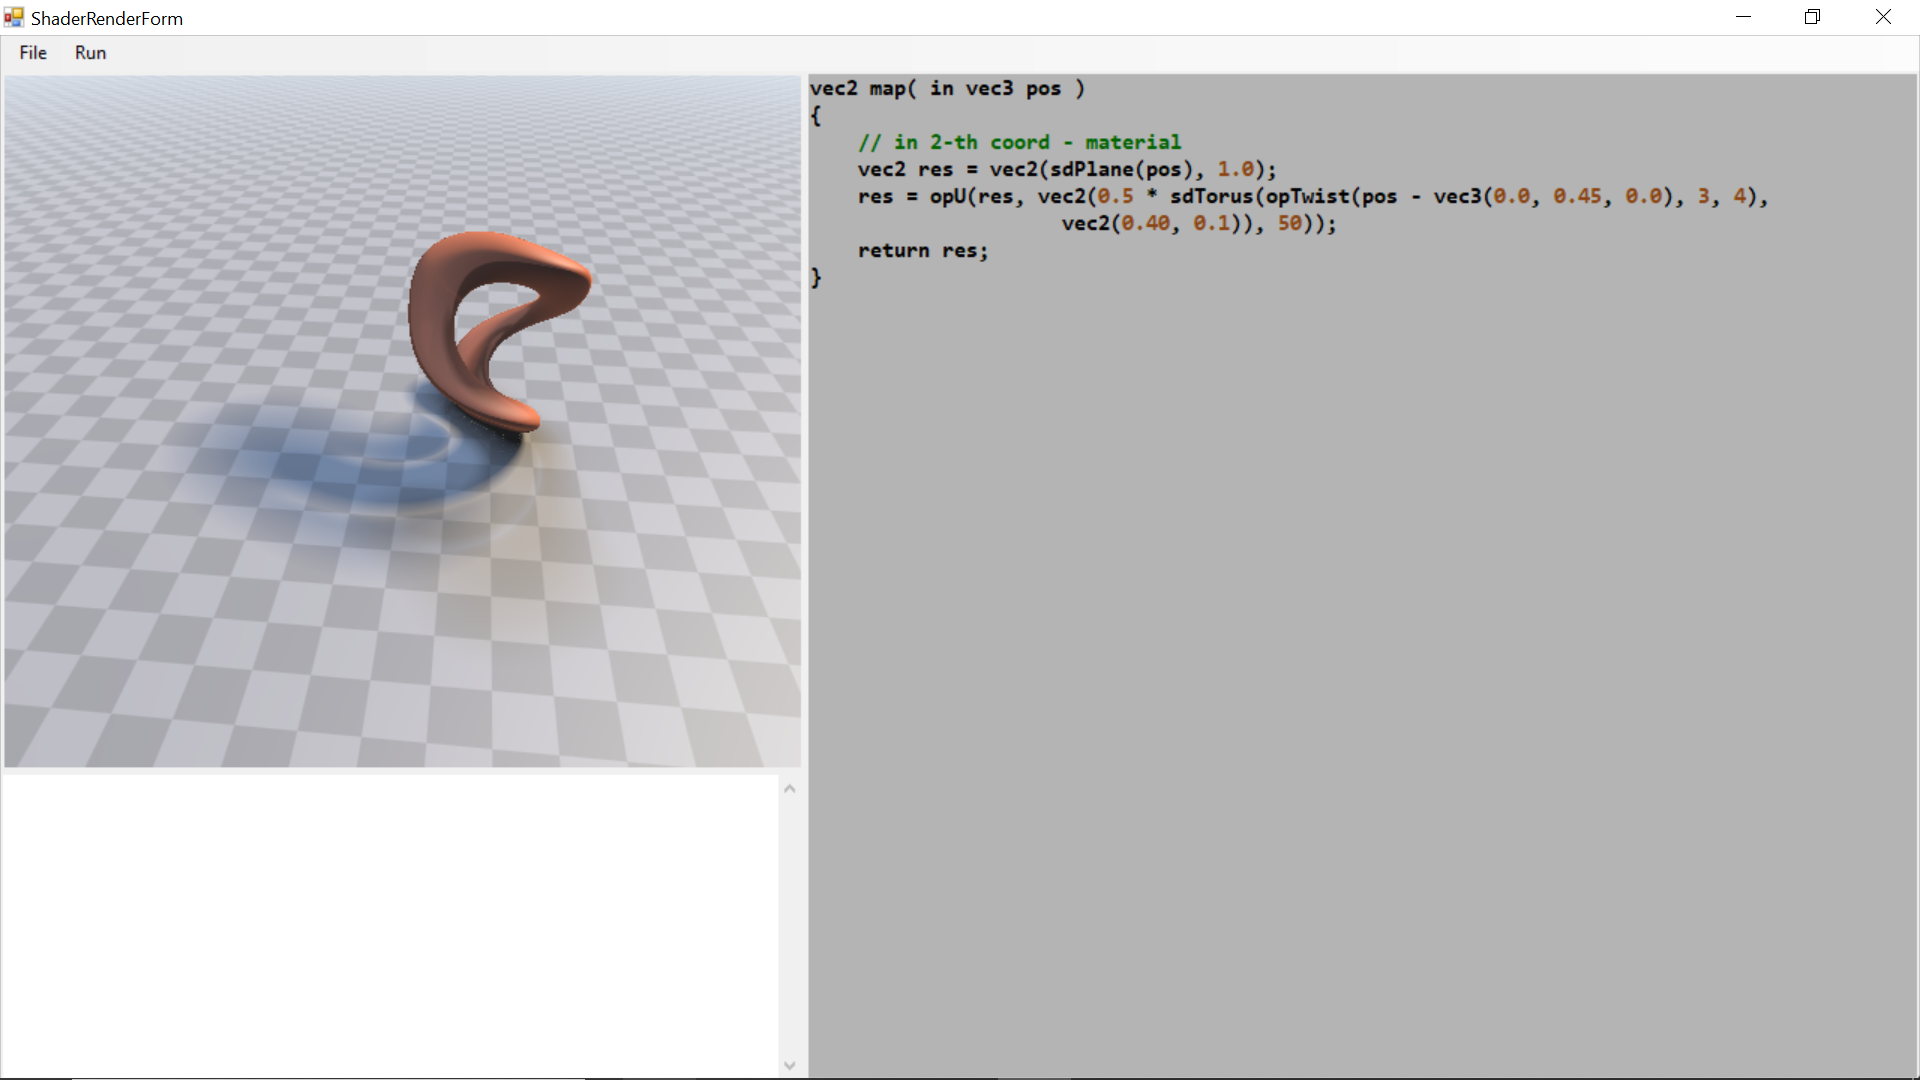
\includegraphics[width = 250pt]{prim1.png}
\caption{Результат действия функции <<opTwist>>, примененной к тору.}
\end{figure}

\section{IDE}
Была реализована IDE для написания своих примеров работы алгоритма RayMarching, а так же небольшая библиотека различных функций. Внутрь IDE добавлена поддержка освещения,
мягких теней и вращения камеры вокруг сцены. Чтобы написать свой пример, необходимо написать функцию map --- функцию, для каждой точки возвращающую
наименьшее расстояние до сцены. Список всех реализованных функций можно посмотреть на Git в файле <<RayMarchBegin.glsl>>.
В самой IDE реализована подсветка синтаксиса, вывод ошибок в специальном окне, если что-то написано неверно, а так же окно с результатом.
Так же для быстродействия данного алгоритма, чтобы сцены могли изменяться в реальном времени, все расчеты выполняются параллельно на графическом процессоре с 
помощью пиксельных шейдеров \cite{wiki:shader}. Примеры работы IDE можно посмотреть выше (рис. 6), (рис.5).
По технической части --- все окна реализованы на C\#, библиотека функций и сам алгоритм реализованы на языке glsl, специальном С-подобном шейдерном языке, исполняемом
на графическом процессоре. 

% У заключения нет номера главы
\section*{Заключение}

Итого было сделано: \\
1) Исследован алгоритм Ray Marching \\
2) Реализован данный алгоритм, а так же реализована библиотека с различными функциями Ray Marching \\
3) Реализована IDE для сцен Ray Marching \\
4) Выполнена оптимизация для выполнения сцен в реальном времени. \\

Проект можно посмотреть в данном репозитории --- \\ <<https://github.com/chudovas/RayMarchIDE>>. 

\setmonofont[Mapping=tex-text]{CMU Typewriter Text}
\bibliographystyle{ugost2008ls}
\bibliography{diploma.bib}
\end{document}
